\documentclass[a4paper,12pt]{article}
\usepackage[margin=1in]{geometry}

\usepackage[T2A]{fontenc}			% кодировка
\usepackage[utf8]{inputenc}			% кодировка исходного текста
\usepackage[english,russian]{babel}	% локализация и переносы
\usepackage{graphicx}                % Математика
\usepackage{amsmath,amsfonts,amssymb,amsthm,mathtools} 
\usepackage{mathtext}
\usepackage[T2A]{fontenc}
\usepackage[utf8]{inputenc}

\usepackage{wasysym}

%Заговолок
\author{Бичина Марина 
группа Б04-005 1 курса ФЭФМ}
\title{}
\date{}


\begin{document} % начало документа

\begin{center}
\begin{Large}
{Корнеев Николай Б04-005, Лабораторная работа № 4.2.3 Интерферометр Релея}
\end{Large}
\end{center}
\paragraph{Цель работы:} 
\begin{enumerate}
\itemsep0em
\item Ознакомиться:

 с интерференцией на двух щелях\\
 устройством и принципом действия интерферометра Релея\\
 с его применением для измерения показателей преломления газов
 \item Исследовать изменение показателя преломления воздуха при изменении давления 
 \item Рассчитать показатели преломления воздуха и углекислого газа при нормальных условиях
\end{enumerate}
\paragraph{Оборудование:}
\begin{enumerate}
\itemsep0em
\item Технический интерферометр ИТР-1
\item Светофильтр
\item Баллон с $CO_2$ 
\item Сильфон
\item Манометр
\item Краны
\end{enumerate}


\paragraph{Теоретическая справка:}
\begin{enumerate}
\itemsep0em
\item Интерференцией называют взаимное увеличение или уменьшение результирующей амплитуды двух или нескольких когерентных волн при их наложении друг на друга. В работе мы используем двухлучевой интерферометр. 
\item Волновые или колебательные процессы называются когерентными, если они протекают согласованно во времени и пространстве: их разность фаз не изменяется во времени.
\item \textbf{Описание установки:}\\
Интерферометр Релея основан на явлении дифракции света на двух параллельных щелях. 
\begin{figure}[h!]
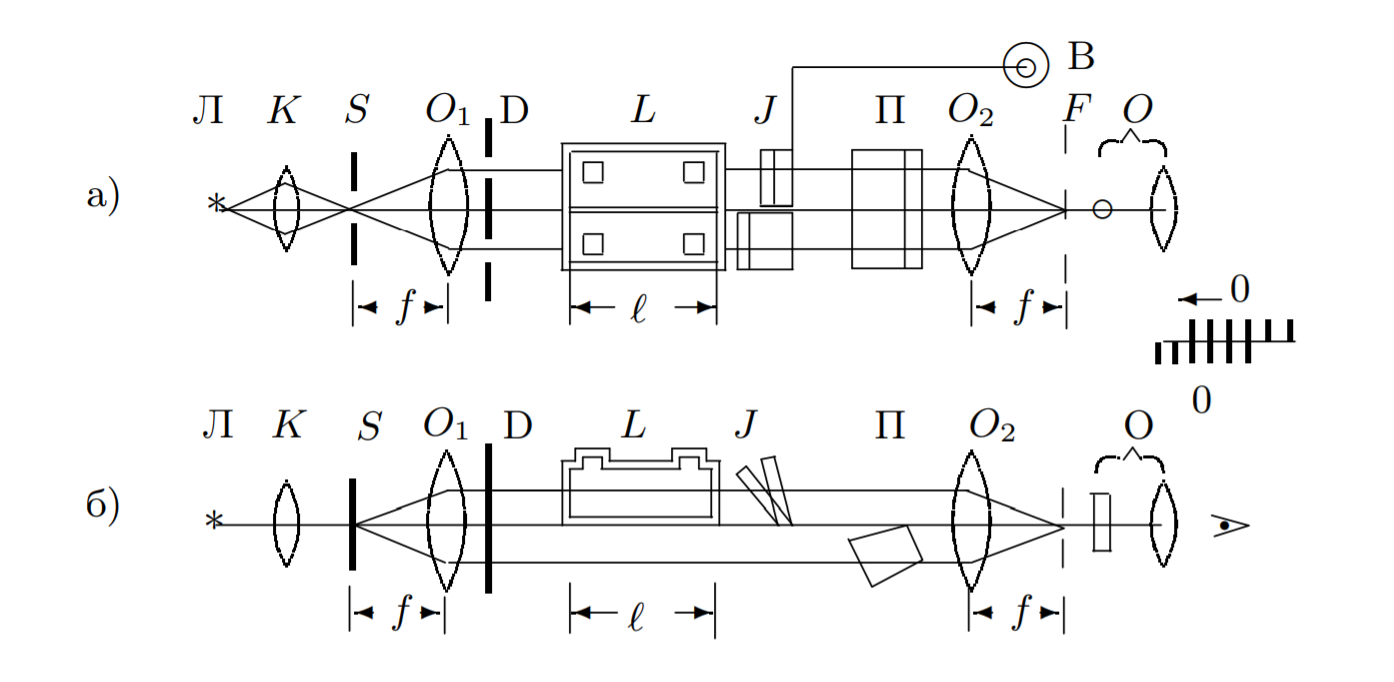
\includegraphics[scale=0.6]{setup.png} 
\caption{Схема установки a) сверху б) сбоку}
\end{figure}
Лампа накаливания Л с помощью конденсора K ярко освещает узкую
входную щель S, расположенную в фокусе объектива $O_1$. \\ Коллиматор, состоящий из щели S и объектива $O_1$, посылает параллельный пучок на диафрагму D с двумя вертикальными
щелями (расстояние между щелями d). Свет после двойной щели проходит кювету L, состоящую из двух одинаковых стеклянных камер, в
которые вводятся исследуемые газы. Кювета занимает только верхнюю часть пространства между
объективами $O_1$ и $O_2$, длина кюветы $l = 25$ см За кюветой расположены две
стеклянные пластинки J  и пластинка П.\\
Интерференционная картина (картина дифракции на двух щелях),
наблюдаемая в фокальной плоскости F объектива $O_2$, представляет собой две системы равноотстоящих полос, параллельных щелям: верхняя образована лучами, прошедшими через кювету, нижняя
(неподвижная) — лучами, прошедшими под кюветой. В установке есть компенсатор Жамена. Данное устройство помогает совместить подвижную и неподвижную системы полос.
\item При малых дифракционных углах $\phi = \lambda/d$ расстояние между соседними светлыми полосами  
\begin{equation}
\delta y = f \frac{\lambda}{d}\
\end{equation}
\begin{equation}
\delta n = k\frac{\lambda}{l}\
\end{equation}
\item Показатель преломления n исследуемого газа определяется путем сравнения с воздухом при атмосферном давлении 
\begin{equation}
n = n_{\text{возд}} +\frac{\Delta}{l}
\end{equation}
\item Зависимость показателя преломления газа от давления и температуры\\
Диэлектрическая проницаемость $\epsilon$ газа невзаимодействующих диполей считается по формуле:
\begin{equation}
\epsilon = n^2 = 1 + N\alpha
\end{equation}
где N - концентрация молекул в газе, $\alpha$ - поляризуемость молекулы. Для разреженных газов справедливо приближение:
$$n - 1 \approx \frac{\alpha}{2kT}P$$
Тогда для разности показателей преломления $
\delta n$ измеряемой с помощью интерферометра Релея и разности давления $
\Delta P$, измеряемой с помощью манометра, имеем соотношения
\begin{equation}
\delta n = \frac{\alpha}{2kT}P\;\;\;\;\;\;\; \frac{dn}{dP} = \frac{\alpha}{2kT}
\end{equation}
\end{enumerate}
\paragraph{Ход работы:}
\begin{enumerate}
\itemsep0em
\item Параметры установки:
\begin{enumerate}
\itemsep0em
\item Длина кюветы $l = 25$ см
\item Длина волны, пропускаемая фильтром $\lambda = 670 \pm 50 $ нм
\item Температура окружающей среды   $T=296$ K
\item Атмосферное давление $P= 99.6$ кПа
\end{enumerate}
\item \textbf{Калибровка}\\
\begin{figure}[h!]
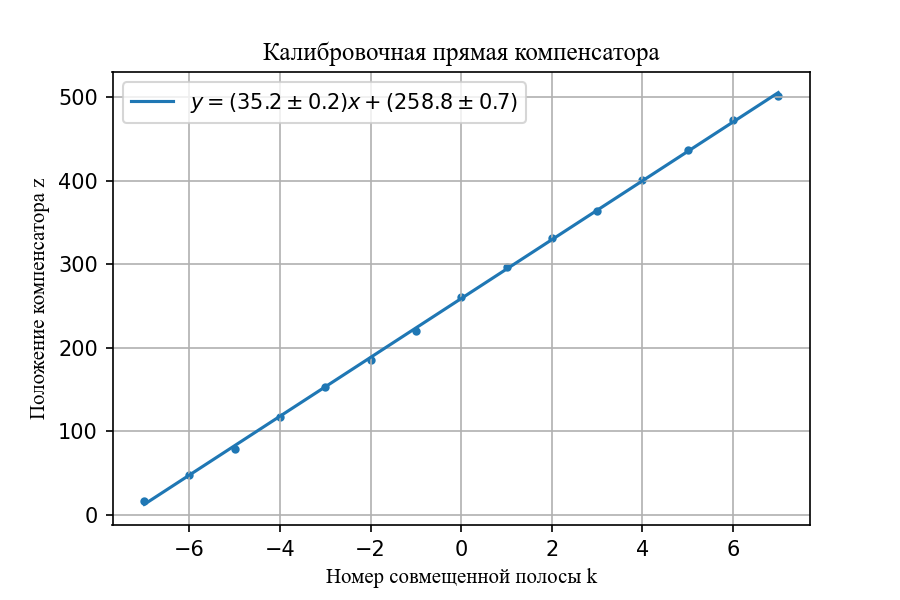
\includegraphics[scale=0.9]{plot_1.png} 
\end{figure} Прокалибруем компенсатор в единицах $\lambda$, выделив узкий интервал длин волн с помощью светофильтра. При калибровке используем все полосы, наблюдаемые в окуляре слева и справа от нулевой полосы\\
\textbf{Построим график зависимости $k(z)$ , пользуясь методом наименьших квадратов $ y = a + bx $}
\begin{equation}
b = \frac{\langle xy \rangle - \langle x \rangle \langle y \rangle}{\langle x^2 \rangle - \langle x \rangle^2} \;\;
a = \langle y \rangle - b \cdot \langle x \rangle
\label{mnk}
\end{equation}
Погрешность в этом случае можно найти по формуле: 
\begin{equation}
\sigma_b \approx \frac{1}{\sqrt{N}}\sqrt{\frac{\langle y^2 \rangle - \langle y \rangle ^ 2}{\langle x^2 \rangle - \langle x \rangle ^ 2} - b^2} ;\;\;\ \sigma_a \approx \sigma_b\sqrt{\langle x^2 \rangle - \langle x \rangle ^2} 
\end{equation}
Тогда коэффициенты а и b равны: 
\[b = 35.2 \pm 0.2\;\;\;\;\;\; a = 258.8 \pm 0.7\] 

\item \textbf{Зависимость $\Delta n(P)$ для воздуха}\\
В одной из кювет находится воздух при атмосферном давлении, в другой -- под давлением. Будем менять давление в пределах от -1000 до 1000 мм вод ст и смещать центральные полосы для каждого значения давлений, в процессе фиксируя положение компенсатора, соответствующее значению давления. Далее, исходя из калибровочного графика рассчитаем разность хода, и по формуле (2) найдем соответствующею величину $\delta n$. Все измеренные и полученные величины занесем в таблицу и по данным построим график зависимости $\Delta n(P)$ для воздуха
\begin{figure}[h!]
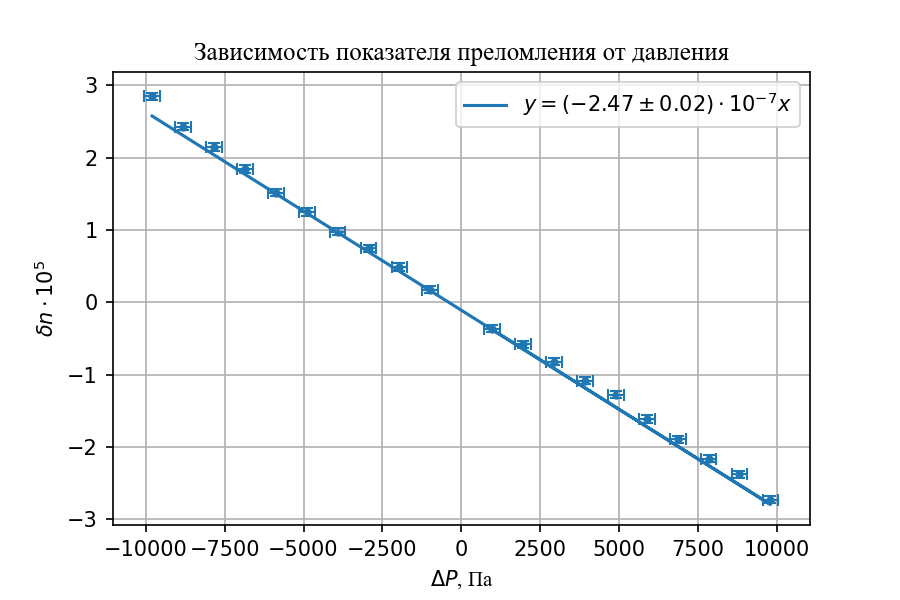
\includegraphics[scale=0.9]{plot_2.png} 
\end{figure}
 На график нанесем кресты погрешностей: Погрешность измерения показателя преломления зависит от погрешности совмещенной полосы k\\
 Тогда по формуле (2) получим погрешность для $\delta n = 5\cdot 10^{-9}$  \\
 Погрешность давления $\Delta P = 250$ Па возникает из-за того, что давление "плывет" и его необходимо поддерживать самостоятельно\\
 Рассчитаем систематическую погрешность:
 $$\varepsilon_{\text{сист}} = \sqrt{(\frac{\Delta\Delta P}{\Delta P})^2 + (\frac{\Delta\delta n}{\delta n})^2}=\sqrt{(\frac{250}{10000})^2 + (\frac{0.5}{25})^2} = 3.2 \%$$
 Тогда коэффициент наклона графика: $(2.47 \pm 0.12) \cdot 10^{-9}$
 \item Рассчитаем среднюю поляризацию молекул воздуха по формуле (5)
 \[\alpha = 2kT\frac{\delta n }{\Delta P} = 2 \cdot\ 1.38\cdot 10^{-23} \cdot 296 \cdot 2.5\cdot 10^{-9}= (2.0\pm 0.1) \cdot 10^{-29}\text{Кл м}\]
 Найдем коэффициент преломления воздуха: 
 \[ n = \sqrt{1 + N\alpha}= \sqrt{1 + 2P\frac{\delta n }{\Delta P}}\approx 1 + P\frac{\delta n }{\Delta P} = 1 + 10^5\cdot 2.5\cdot 10^{-9} =1.00025 \pm 0.00001\]
 Получим весьма близкое к табличному значение для коэффициента преломления воздуха
 \item \textbf{Показатель преломления СO$_2$}
 В одной из кювет будет находиться воздух при атмосферном давлении, в другой -- углекислый газ под атмосферным давлением. Сначала будем просто напускать газ и следить за смещением интерференционной картины, а когда она перестанет смещаться, зафиксируем положение компенсатора. Далее пронаблюдаем за смещением спектральной картины, фиксируя положение компенсатора и момент времени с остановки напускания углекислого газа. По формуле (2) также найдем $\delta n$\\
 По начальному положению компенсатора вычислим показатель преломления углекислого газа.

$$n_{CO_2} = n_{\text{возд} }+\delta n = 1.00025 + 0.00016 = 1.00041$$
Тогда погрешность суммы:
$$ \sigma n_{CO_2} = \sqrt{0.00001^2 + 0.0000027^2}\approx 0.00001$$
Тогда:
$$n_{CO_2} = 1.00041 \pm 0.00001$$ 
\item \textbf{Диапазон измерений интерферометра}
Диапазон допустимых для измерения интервалось коэффициента преломления снизу ограничен погрешностью $\delta n = 2.8 \cdot 10^{-6}$, а сверху -- порядком $
\delta n = 10^4$
\end{enumerate}
\paragraph{Выводы:}
\begin{enumerate}
\item Ознакомились с принципом работы с интерференцией на двух щелях на примере установки Релея
\item Установили линейную природу изменения показателя преломления воздуха при изменении давления (см график 2)
\item Получили значения показателя преломления для воздуха и углекислого газа: 
\begin{equation*}
\delta n_{\text{возд}} = 1.00025 \pm 0.00001\;\;\;\;\;\;\;\; \delta n_{CO_2} = 1.00041 \pm 0.00001
\end{equation*}
При табличных значениях: 
\begin{equation*}
\delta n_{\text{возд}} = 1,00029\;\;\;\;\;\;\;\;\delta n_{CO_2} = 1,00045
\end{equation*}
\item Нашли среднюю поляризацию воздуха $\alpha = (2.0 \pm 0.1)\cdot 10^{-29}$ Кл м 
\item Оценили диапазон измерений интерферометра Релея
\end{enumerate}
\end{document}